\subsection{Introducción}

Go.JS \cite{gojs} es una biblioteca de JavaScript para implementar editores gráficos dentro de interfaces web. GoJS facilita la implementación de funciones tales como definición de símbolos gráficos, gestión de paletas de símbolos, arrastrar y soltar (\emph{drag and drop}), copiar y pegar, edición de etiquetas de texto asociadas a símbolos gráficos, menús contextuales, función de deshacer o gestión de eventos, entre muchas otras funcionalidades.

Para ilustrar el funcionamiento de GoJS, a continuación, se muestra un ejemplo sencillo de creación de editor gráfico de grafos para el dibujo de círculos interconectados por flechas. Dicho editor se muestra en la Figura~\ref{fig:gojssample}.

\begin{figure}[!tb]
	\centering
	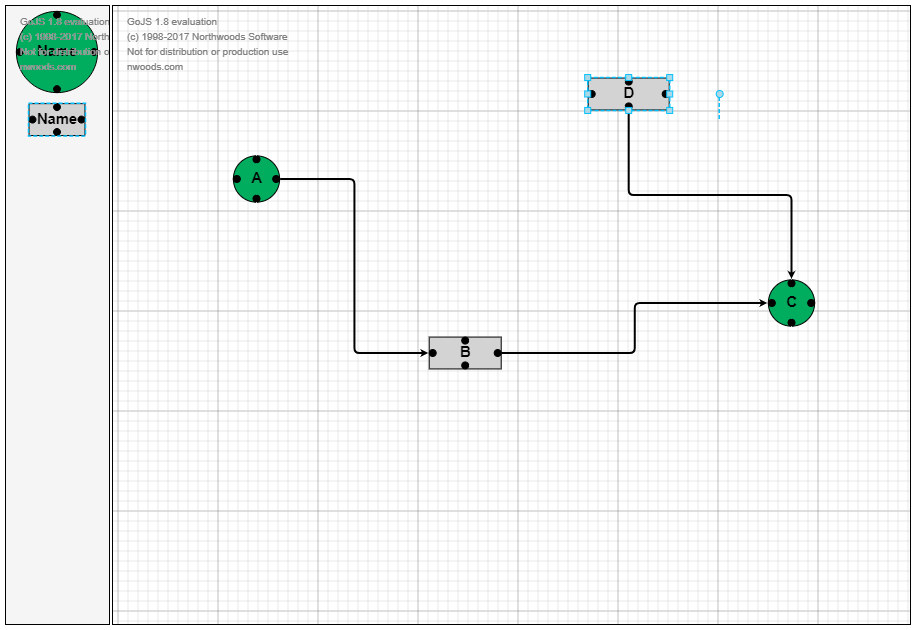
\includegraphics[scale=0.5]{gojssample.png}
	\caption{Editor gráfico creado en GoJS}
    \label{fig:gojssample}
\end{figure}

Para comenzar explicando el ejemplo, cabe destacar que, es necesario reservar dos secciones de la página HTML que lo contiene. Una sección para la paleta contenedora de los elementos gráficos del editor, que en este caso es sólo el círculo, y otra sección para el diagrama sobre el que se depositarán los elementos gráficos. 


\begin{figure}[!tb]
	\centering
	\begin{lstlisting}[language=JavaScript]
	myDiagram =
		$(go.Diagram, "myDiagramDiv",  
		{
			grid: $(go.Panel, "Grid",
				$(go.Shape, "LineH", { stroke: "lightgray", strokeWidth: 0.5 }),
				$(go.Shape, "LineH", { stroke: "gray", strokeWidth: 0.5, interval: 10 }),
				$(go.Shape, "LineV", { stroke: "lightgray", strokeWidth: 0.5 }),
				$(go.Shape, "LineV", { stroke: "gray", strokeWidth: 0.5, interval: 10 })
			),
			allowDrop: true,         
		}
	);
	\end{lstlisting}
	\caption{Creación de un Diagrama}
	\label{fig:creacionDiagrama}
\end{figure}



A continuación, se debe realizar una serie de acciones a nivel de Javascript para proporcionar tanto a la paleta de dibujo, como al área de dibujo del comportamiento deseado. En primer lugar, crearemos una variable \texttt{\$} que dé acceso al entorno GoJS. Esto se realiza mediante la llamada a la sentencia \texttt{make} de librería \emph{GraphObject} de GoJS (Figura~\ref{fig:asignacionDollar},~Línea 1).

\begin{figure}[!tb]
	\centering
	\begin{lstlisting}[language=JavaScript]
	var $ = go.GraphObject.make;
	\end{lstlisting}
	\caption{Asignación de la variable \texttt{\$}}
	\label{fig:asignacionDollar}
\end{figure}

Seguidamente, se personaliza la sección HTML reservada al diagrama, denominada \texttt{myDiagramDiv} (Figura~\ref{fig:creacionDiagrama},~Líneas~01-13), asignándole un \emph{grid} o cuadrícula de fondo (Figura~\ref{fig:creacionDiagrama},~Líneas~04-09), especificando los colores de las líneas de la cuadrícula(mediante la propiedad \emph{stroke})  y dándole la capacidad de poder arrastrar elementos sobre él (Figura~\ref{fig:creacionDiagrama},~Línea 10).

%%========================================================================%%
%% NOTE(Pablo): Hasta aquí va más o menos bien la cosa, pero aquí         %%
%%    empezamos a perder el hilo. ¿De dónde han salido los círculos y     %%
%%    qué es un puerto. Lo normal es explicar primero cómo se añaden      %%
%%    círculos a la paleta, qué es un puerto, la necesidad de crearlos,   %%
%%    y luego ya cómo se crean.                                            %% 
%%========================================================================%%
\begin{figure}[!tb]
	\centering
	\begin{lstlisting}[language=JavaScript]
	myDiagram.nodeTemplate =
		$(go.Node, "Spot",
		{ locationSpot: go.Spot.Center },
		new go.Binding("location").makeTwoWay(go.Point.stringify),
		{ selectable: true, selectionAdornmentTemplate: nodeSelectionAdornmentTemplate },
		{ resizable: true, resizeObjectName: "PANEL", resizeAdornmentTemplate: nodeResizeAdornmentTemplate },
		{ rotatable: true, rotateAdornmentTemplate: nodeRotateAdornmentTemplate },
	
		$(go.Panel, "Auto",
		{ name: "PANEL" },
		$(go.Shape,  
		{
			portId: "", 
			fromLinkable: true, toLinkable: true, cursor: "pointer",
		},
			new go.Binding("figure"),
			new go.Binding("fill")),
		$(go.TextBlock,
		{
			maxSize: new go.Size(50, 50),
			editable: true
		},
		new go.Binding("text").makeTwoWay())
		)
	);
	\end{lstlisting}
\caption{Declaración del patrón del Nodo}
\label{fig:patronNodo}
\end{figure}

La Figura~\ref{fig:patronNodo} muestra cómo se crea el patrón, o comúnmente conocido \emph{template\footnote{El template declara el conjunto de características y/o directrices que acompañan a un nodo en su creación, por ejemplo se puede definir un color concreto, o unas características que pueden ser modificadas.}}, que servirán de esqueleto para los \emph{nodos} de un diagrama. Los nodos son todos aquellos elementos de los que se va a componer el diagrama. En nuestro ejemplo, estos nodos serán círculos y rectángulos. Para crear la definición un nodo lo primero es declarar el nodo con \texttt{\$(go.Node} (Figura~\ref{fig:patronNodo},~Línea~2). 

A continuación, especificamos, mediante la definición de ciertas propiedades, cómo se comportará el nodo (Figura~\ref{fig:patronNodo},~Líneas~05-24). En nuestro caso, se indica que, dentro de las caracteristicas del nodo, podrá ser seleccionado, redimensionado y rotado (Figura~\ref{fig:patronNodo},~Líneas~05-07), además, se ha establecido una localización o situación de los puntos por defecto centrada (Figura~\ref{fig:patronNodo},~Línea~03). Junto a ella, aparece una sentencia  \emph{binding} (Figura~\ref{fig:patronNodo},~Línea~04), esta sentencia sirve para permitir en un futuro modificar dicha propiedad.

Al crear un nodo, se reserva un espacio sobre el que se van a situar los diferentes elementos del nodo, basándonos en el ejemplo, este nodo contiene un \emph{panel}(Figura~\ref{fig:patronNodo}, Línea~09), que actúa como contenedor de la figura o \emph{shape}(Figura~\ref{fig:patronNodo},~Línea~11), que es la encargada de definir la forma y otras características del nodo, como es el puerto del nodo (que actúa como identificador)(Figura~\ref{fig:patronNodo},~Línea~13) y las propiedades de enlace de las que se hablarán más adelante (Figura~\ref{fig:patronNodo},~Línea~14). En nuestro caso, dicho panel tendrá la capacidad de poseer diferentes formas (como serán el circulo y el rectángulo) y colores gracias a los \emph{bindings} (Figura~\ref{fig:patronNodo},~Líneas~16-17). Además poseerá una etiqueta de texto que permitirá especificar su nombre, que tambien podrá ser modificada(Figura~\ref{fig:patronNodo},~Líneas~18-24).

Una vez definidas las propiedades básicas de un nodo, el siguiente paso es definir cómo enlazar dichos nodos. Para ello debemos definir dos elementos: \emph{puertos\footnote{En la Figura~\ref{fig:gojssample}, aparecen como unos círculos negros en los ejes de las figuras.}} y \emph{enlaces\footnote{Son los links o uniones entre nodos, los cuales se conectan entre sí a partir de los puertos.}}. Los puertos de un nodo son los puntos de unión a los enlaces. 

\begin{figure}[!tb]
	\centering
	\begin{lstlisting}[language=JavaScript]
	function makePort(name, spot) {
		return $(go.Shape, "Circle",
		{
			desiredSize: new go.Size(7, 7),
			alignment: spot,  
			alignmentFocus: spot,  
			portId: name,  
			fromLinkable: true, toLinkable: true,  
			cursor: "pointer"  
		});
	}
	\end{lstlisting}
	\caption{Función MakePort}
	\label{fig:funcionMakeport}
\end{figure}
	
Para añadir puertos a los nodos se ha creado una función una función llamada \emph{makePort}, la cual se muestra en la Figura~\ref{fig:funcionMakeport}. En este fragmento de código se define un puerto, como una forma circular, al que se le establece un identificador(Figura~\ref{fig:funcionMakeport},~Línea~07), una posición(Figura~\ref{fig:funcionMakeport},~Líneas~05-06) y un tamaño (Figura~\ref{fig:funcionMakeport},~Línea~04).



\begin{figure}[!tb]
	\centering
	\begin{lstlisting}[language=JavaScript]
	myDiagram.nodeTemplate =
		$(go.Node, "Spot",
		{ locationSpot: go.Spot.Center },
		new go.Binding("location").makeTwoWay(go.Point.stringify),
		{ selectable: true, selectionAdornmentTemplate: nodeSelectionAdornmentTemplate },
		{ resizable: true, resizeObjectName: "PANEL", resizeAdornmentTemplate: nodeResizeAdornmentTemplate },
		{ rotatable: true, rotateAdornmentTemplate: nodeRotateAdornmentTemplate },
		
			$(go.Panel, "Auto",
			{ name: "PANEL" },
				$(go.Shape,  
				{
					portId: "", 
					fromLinkable: true, toLinkable: true, cursor: "pointer",
				},
				new go.Binding("figure"),
				new go.Binding("fill")),
					$(go.TextBlock,
					{
						maxSize: new go.Size(50, 50),
						editable: true
					},
					new go.Binding("text").makeTwoWay()
					)
			),
		makePort("T", go.Spot.Top),
		makePort("L", go.Spot.Left),
		makePort("R", go.Spot.Right),
		makePort("B", go.Spot.Bottom)
	);
	
	\end{lstlisting}
	\caption{Patrón Nodo con Puertos}
	\label{fig:patronNodoFinal}
\end{figure}


A continuación, con la explicación previa sobre cómo se crea un puerto,  añadimos cuatro llamadas a esta función dentro del patrón del nodo, con el objeto de crear un puerto a cada lado del eje del mismo (Figura~\ref{fig:patronNodoFinal},~Línea~04), quedando una definitiva especificación de esta.


\begin{figure}[!tb]
	\centering
	\begin{lstlisting}[language=JavaScript]
	myDiagram.linkTemplate =
		$(go.Link, 
			$(go.Shape,  
			{ isPanelMain: true, strokeWidth: 2 }),
			$(go.Shape,  
			{ toArrow: "Standard", stroke: null }
		)
	)
	\end{lstlisting}
\caption{Declaración del patrón del Link}
\label{fig:patronlink}
\end{figure}

Una vez definidos los puertos, especificamos cómo se comportarán los enlaces entre nodos, tal como muestra la Figura~\ref{fig:patronlink}. En esta figura se declara al link como dos shapes (uno principal y otro secundario) que definirán el grosor del link y establecerán una flecha al final del mismo respectivamente (Figura~\ref{fig:funcionMakeport},~Líneas~03-06).


\begin{figure}[!tb]
	\centering
\begin{lstlisting}[language=JavaScript]
myPalette =
	$(go.Palette, "myPaletteDiv",  
	{
		nodeTemplateMap: myDiagram.nodeTemplateMap,  
		model: new go.GraphLinksModel([  
			{ text: "Name", figure: "Circle", fill: "#00AD5F" },
			{ text: "Name", figure: "Rectangle", fill: "lightgray" }
			])
		}
);
\end{lstlisting}
\caption{Creación de la Paleta de Nodos}
\label{fig:paletaNodos}
\end{figure}

Por último, se procede a crear la paleta que contendrá los círculos y rectángulos, tal como se muestra en la Figura~\ref{fig:paletaNodos}. Como se puede observar, la paleta se sitúa sobre una sección HTML denominada \emph{myPalleteDiv}, la cual fue reservada con anterioridad. 

Centrándonos en las características o el propio patrón, se puede observar que para la definición de los nodos que estarán dentro de la paleta se ha utilizado el mismo patrón creado para los nodos(Figura~\ref{fig:paletaNodos},~Línea~04). Y por último se le declara el modelo, que es el conjunto de figuras que poseerá dicha paleta, para ello se crean objetos siguiendo el patrón del nodo, en un primer caso tenemos el circulo con un color verde (Figura~\ref{fig:paletaNodos},~Línea~06) y en un segundo caso tenemos el rectángulo con un color gris (Figura~\ref{fig:paletaNodos},~Línea~07), ambos con un nombre por defecto en su interior que podrá ser editado.


Una vez definidos estos elementos, nuestro editor gráfico queda implementado, y GoJS se encargará de dibujar la paleta y el diagrama, así como de pintar los elementos sobre el área de dibujo cuando estos son seleccionados en la paleta, permitiendo arrastrarlos, redimensionarlos o renombrarlos, entre otras funciones. 
